\section{Introduction}
Several discretization methods haven been developed for arbitrary polygonal
meshes \cite{pwld_2d,pwld_3d,pwl_diffusion,palmer_ane,palmer_proc,palmer_fe,
wachspress,cell_centered_diff,mimetic}.  Using polygonal
cells can be advantageous because the number of unknowns can be reduced while
maintaining symmetry within the mesh. This potential reduction in 
number of unknowns can be seen by comparing a hexagonal cell with a triangular
discretization of the same area:
\begin{figure}[H]
\centering
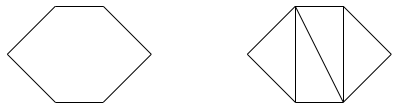
\includegraphics[width=0.5\textwidth]{hex_tri_cells}
\caption{Hexagonal cell versus triangle cells.}
\end{figure}
If there is one unknown per vertex, the hexagonal cell will have only six
unknowns compared to the 12 unknowns of the triangular discretization. Another 
advantage of polygonal cells is that they can be used for adaptive mesh refinement 
(AMR) \cite{amr_rad,amr_block,amr_unstruc} without having to
deal with hanging nodes \cite{arbitrary_hanging_nodes,dealII_hanging_nodes,
locally_hanging_nodes}. On the figure below, the left cell is a pentagon whereas 
the two cells on the right are quadrilaterals:
\begin{figure}[H]
\centering
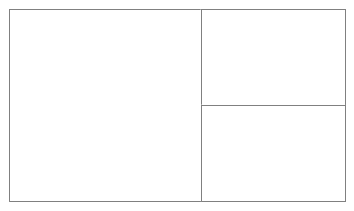
\includegraphics[width=0.3\textwidth]{amr}
\caption{AMR mesh.}
\end{figure}
The PieceWise Linear Discontinuous (PWLD) finite elements \cite{pwld_2d,pwld_3d} 
have been successfully used to solve the transport equation on arbitrary
polygonal meshes. PieceWise Linear Continuous finite elements have been used to 
discretize the diffusion equation and have shown to be second order and to
produce a symmetric positive (SPD) matrix \cite{pwl_diffusion}. However, no 
Diffusion Synthetic Acceleration (DSA) \cite{dsa_ref} was developed using this 
discretization and to the best of our knowledge, there is no DSA for arbitrary
polygonal mesh. In this work, we remedy this lack by adapting the Modified Interior 
Penalty (MIP) DSA developed in \cite{mip} for triangular cells. By using PWLD 
finite elements with MIP, MIP will be able to work on arbitrary polygonal 
cells. Since MIP produces SPD equations, it has usually 
been solved using conjugate gradient (CG) preconditioned by SSOR. In this
article, the effectiveness of algebraic multigrid methods (AMG) to precondition 
the Krylov solver \cite{amg,amg_course} will be tested. Algebraic multigrid methods 
allow to use multigrid techniques when there is no grid or when the mesh is 
unstructured. Instead of using a succession of grids based on the geometry of the 
problems, the grids are based on properties of the matrix. Therefore, AMG can
be used as black-box solver or preconditioner.

The remainder of this paper is organized as follows. In Sec.(\ref{sec_mip}),
we introduce the PWLD finite elements and we adapt MIP to this discretization. 
In Sec.(\ref{sec_amg}), we briefly explain AMG and we introduce the two different 
AMG methods that we will use, the ML package of Trilinos \cite{ml_guide} and the 
AGMG (AGgregation-based algebraic MultiGrid) code \cite{agmg_guide}. In 
Sec.(\ref{sec_res}), we show the Fourier analysis of MIP discretized with PWLD
and we compare the different preconditioners of the CG solver. In 
Sec.(\ref{sec_conc}), we give our conclusions.
